\documentclass[12pt]{article}
\usepackage[a4paper, total={6in, 10in}]{geometry}
\usepackage{amsmath}
\usepackage{graphicx}
\usepackage{hyperref}
\usepackage[latin1]{inputenc}

\DeclareMathOperator{\PAR}{PAR}
\DeclareMathOperator{\PARMAX}{PAR_{MAX}}
\DeclareMathOperator{\dB}{dB}

\title{Basic Amplitude Modulation theory [DRAFT]}
\author{heso}
\date{\today}

\begin{document}
\maketitle

\section{Single-channel AM}

A basic expression for a general sinusoidally AM-modulated RF signal $S_{RF}(t)$ can be written as:
\begin{equation}
S_{RF}(t)  = A \sin(\omega_c t) \left( 1 + m \sin(\omega_m t) \right) \\
\end{equation}
where $A$ is the amplitude, $\omega_c$ is the carrier (angular) frequency, $m$ is the modulation index and $\omega_m$ is the modulation frequency.

Using trigonometric identities, this expression can be rewritten as
\begin{equation}
\begin{aligned}
S_{RF}(t) & = A \sin(\omega_c t) + m A \sin(\omega_c t) \sin(\omega_m t) \\
      & = A \sin(\omega_c t) + 
    m \frac{A}{2} ( \cos((\omega_c - \omega_m)t) - \cos((\omega_c + \omega_m)t) )
\end{aligned}
\end{equation}
The first term is the carrier, the second the lower sideband (LSB), and the third term the upper sideband (USB).

So modulation index can be calculated from 
\begin{equation}
\begin{aligned}
m &= 2 \frac{\max{ \{ V_{LSB} \} }}{\max{ \{ V_C \} }} \\
&= 2 \frac{\max{ \{ V_{USB} \} }}{\max{ \{ V_C \} }} \\
\end{aligned}
\end{equation}


\subsection{Average power}

Since the RMS of a sine wave $ A \sin(\omega t)$ is RMS$\{A\sin(\omega t)\} = A / \sqrt{2}$, we have the following expression for average carrier power $P_C$ (in a 1 $\Omega$ system):
\begin{equation}
\begin{aligned}
P_{C,avg} & = \frac{A^2}{2}
\end{aligned}
\end{equation}
Similarly, for upper and lower sideband average power $P_{USB}$ and $P_{LSB}$: 
\begin{equation}
\begin{aligned}
P_{USB,avg} & = P_{LSB,avg} \\
      & = \frac{m^2}{2} \frac{A^2}{4}
\end{aligned}
\end{equation}

Using the above equations, the total average power $P_{avg}$ of $S_{RF}(t)$ can be rewritten as
\begin{equation}
\begin{aligned}
P_{avg} & = P_{C,avg} + P_{USB,avg} + P_{LSB,avg} \\
        & = P_{C,avg} (1 + \frac{m^2}{2})
\end{aligned}
\end{equation}

\subsection{Peak power}

For the peak (instantaneous) power $P_{pk}$ of $S_{RF}(t)$, it is obtained at the instant $S_{RF}(t)$ reaches its peak value, i.e. where sinusoids reach $\pm 1$:
\begin{equation}
\begin{aligned}
P_{pk} & = \max \{ S_{RF}(t) \}^2 \\
        & =  \{ A ( 1 + m ) \}^2 \\
        & =  A^2 ( 1 + m )^2 \\
        & =  P_{C,avg} \times 2 ( 1 + m )^2 \\
        & =  P_{C,pk} \times ( 1 + m )^2 \\
\end{aligned}
\end{equation}

Note the difference between peak power and peak envelope power. Peak Envelope Power (PEP) is "the average power supplied to the antenna by a transmitter during one radio-frequency cycle at the crest of the modulation envelope taken under normal operating conditions".

PEP is by definition half of the peak (instantaneous) power. 

\subsection{PAR}

\begin{equation}
\begin{aligned}
\PAR     & =  \frac{P_{pk}}{P_{avg}} \\
        & =  \frac{A^2 ( 1 + m )^2 }{\frac{A^2}{2}  ( 1 + m^2 / 2)} \\
        & =  2 \frac{( 1 + m )^2 }{ 1 + m^2 / 2} \\
\end{aligned}
\end{equation}

\subsection{Voice}

It has been simulated that voice AM with modulation index 0.85 can be emulated as sinusoidal AM with modulation index m around 0.28, as far as average power is concerned. Denoting ordinary modulation index as $m_{peak} = 0.85$, and the average modulation index $m_{avg} = 0.28$, the expression for PAR becomes
\begin{equation}
\begin{aligned}
\PAR   & = 2 \frac{( 1 + m_{pk} )^2 }{ 1 + m_{avg}^2 / 2} \\
       & = 2 \frac{( 1 + 0.85 )^2 }{ 1 + 0.28^2 / 2} \\
       & \approx 6.59 \ (\sim 8.2 \dB)
\end{aligned}
\end{equation}
This has been verified by simulations.

\section{Multi-channel AM}

This section deals with multi-channel AM, i.e. different AM channels.

\subsection{Average power}

Average power of a N-channel AM signal is simply the added power of each channel:
\begin{equation}
\begin{aligned}
P_{avg}(N) & = \sum_{i=1}^{N}  P_{C,avg,i} \\
        & = \sum_{i=1}^{N} A_i (1 + \frac{m_i^2}{2})
\end{aligned}
\end{equation}
So for same amplitude A and modulation index m, we have
\begin{equation}
\begin{aligned}
P_{avg}(N) & = \sum_{i=1}^{N} A (1 + \frac{m^2}{2}) \\
           & = N \cdot A (1 + \frac{m^2}{2}) \\
           & = N \cdot P_{avg}(1) \\
\end{aligned}
\end{equation}

\subsection{Peak power}

Peak (instantaneous) power occurs when sum of amplitudes of each channel maximizes, with the theoretical value $A_1(1+m_1) + ... + A_N(1+m_N)$. This translates into a peak power value of
\begin{equation}
\begin{aligned}
P_{pk}(N) & = ( \sum_{i=1}^{N}  A_i ( 1 + m_i ) )^2 \\
\end{aligned}
\end{equation}
And so for same amplitude A and modulation index m
\begin{equation}
\begin{aligned}
P_{pk}(N) & = ( N A (1 + m) )^2 \\
       & = N^2 A^2 (1 + m)^2 \\
       & = N^2 P_{pk}(1) \\
\end{aligned}
\end{equation}
This should be understood as a "peak-of-peaks", i.e. an upper bound for peak power. 

\subsection{PAR}

\begin{equation}
\begin{aligned}
\PARMAX(N)  & =  \frac{P_{pk}(N)}{P_{avg}(N)} \\
        & =  \frac{N^2 A^2 ( 1 + m )^2 }{N \frac{A^2}{2}  ( 1 + m^2 / 2)} \\
        & =  2 N \frac{( 1 + m )^2 }{ 1 + m^2 / 2} \\
        & =  N \cdot \PAR(1) \\
\end{aligned}
\end{equation}


\section{Compression}

\subsection{Compression model}
Compression is modelled through an amplitude compressing function of the form
\begin{equation}
\begin{aligned}
f\left(x\right)=x-\alpha x^3
\end{aligned}
\end{equation}
with $\alpha$ being positive.
To find from $\alpha$ from $IIP_3$ [explain]:
\begin{equation}
\begin{aligned}
\alpha = \frac{4}{3\left(IIP_3\right)^2}
\end{aligned}
\end{equation}


\subsection{Compression of AM}

Inserting into the compression function yields:
\begin{equation}
\begin{aligned}
f(A \sin(\varphi_c) \left( 1 + m \sin(\varphi_m) \right))   = & \ A \sin(\varphi_c) \left( 1 + m \sin(\varphi_m) \right) \\
          & - \alpha ( A \sin(\varphi_c) \left( 1 + m \sin(\varphi_m) \right) )^3 \\
          = & A \sin(\varphi_c) \left( 1 + m \sin(\varphi_m) \right)) \\
            & - \alpha A^3 ( \sin(\varphi_c) (1+ m \sin(\varphi_m) ) )^3 \\
\end{aligned}
\end{equation}

To proceed, it is noted that 
\begin{equation}
\begin{aligned}
\Big(\sin(x) (1 + k\sin(y)) \Big)^3 = & \ \frac{1}{32} (-3 k^3 \cos(x - 3 y) + k^3 \cos(3 x - 3 y) \\
 & + 9 k^3 \cos(x - y) - 3 k^3 \cos(3 x - y) - 9 k^3 \cos(x + y) \\
 & + 3 k^3 \cos(3 x + y) + 3 k^3 \cos(x + 3 y) - k^3 \cos(3 x + 3 y) \\
 & - 18 k^2 \sin(x - 2 y) + 6 k^2 \sin(3 x - 2 y) - 18 k^2 \sin(x + 2 y) \\
 & + 6 k^2 \sin(3 x + 2 y) + 36 k^2 \sin(x) - 12 k^2 \sin(3 x) \\
 & + 36 k \cos(x - y) - 12 k \cos(3 x - y) - 36 k \cos(x + y) \\
 & + 12 k \cos(3 x + y) + 24 \sin(x) - 8 \sin(3 x))
\end{aligned}
\end{equation}
Setting $x = \varphi_c = \omega_c t$, $y = \varphi_m = \omega_m t$ and $k=m$, and neglecting terms that do not fall close to $1 \times \omega_c$ yields
\begin{equation}
\begin{aligned}
\Big(\sin(\varphi_c) (1 + m\sin(\varphi_m)) \Big)^3 = & \ \frac{1}{32} \Big(-3 m^3 \cos(\varphi_c - 3 \varphi_m) + 9 m^3 \cos(\varphi_c - \varphi_m) \\
 & - 9 m^3 \cos(\varphi_c + \varphi_m) + 3 m^3 \cos(\varphi_c + 3 \varphi_m)  \\
 & - 18 m^2 \sin(\varphi_c - 2 \varphi_m)  - 18 m^2 \sin(\varphi_c + 2 \varphi_m) \\
 &  + 36 m^2 \sin(\varphi_c) + 36 m \cos(\varphi_c - \varphi_m) \\
 & - 36 m \cos(\varphi_c + \varphi_m) + 24 \sin(\varphi_c) \Big) \\
= & \ \frac{1}{32} \Big( \\
& -3 m^3 \cos(\varphi_c - 3 \varphi_m) \\
& -18 m^2 \sin(\varphi_c - 2 \varphi_m) \\
& + (9 m^3 + 36m) \cos(\varphi_c - \varphi_m) \\
& + (36 m^2 +24)\sin(\varphi_c) \\
& - (9 m^3 +36 m) \cos(\varphi_c + \varphi_m) \\
& - 18 m^2 \sin(\varphi_c + 2 \varphi_m) \\
& + 3 m^3 \cos(\varphi_c + 3 \varphi_m) \Big)
\end{aligned}
\end{equation}
So returning to Equation (17) again,
\begin{equation}
\begin{aligned}
f(A \sin(\varphi_c) \left( 1 + m \sin(\varphi_m) \right))   = & A \sin(\varphi_c) \left( 1 + m \sin(\varphi_m) \right)) \\
            & - \alpha A^3 ( \sin(\varphi_c) (1+ \sin(\varphi_m) ) )^3 \\
            = &  A \sin(\varphi_c) + 
    m \frac{A}{2} ( \cos(\varphi_c - \varphi_m) - \cos(\varphi_c + \varphi_m) \\
            & - \frac{\alpha A^3}{32} \Big( \\
& -3 m^3 \cos(\varphi_c - 3 \varphi_m) \\
& -18 m^2 \sin(\varphi_c - 2 \varphi_m) \\
& + (9 m^3 + 36m) \cos(\varphi_c - \varphi_m) \\
& + (36 m^2 +24)\sin(\varphi_c) \\
& - (9 m^3 +36 m) \cos(\varphi_c + \varphi_m) \\
& - 18 m^2 \sin(\varphi_c + 2 \varphi_m) \\
& + 3 m^3 \cos(\varphi_c + 3 \varphi_m) \Big) \\
=  
& -3 m^3 \cos(\varphi_c - 3 \varphi_m) \\
& -18 m^2 \sin(\varphi_c - 2 \varphi_m) \\
& + \Big( m\frac{A}{2} - \alpha A^3 \frac{9 m^3 + 36m}{32} \Big) \cos(\varphi_c - \varphi_m) \\
& + \Big( A - \alpha A^3 \frac{36 m^2 +24}{32} \big) \sin(\varphi_c) \\
& - \Big( m\frac{A}{2} - \alpha A^3 \frac{9 m^3 + 36m}{32} \Big) \cos(\varphi_c + \varphi_m) \\
& - 18 m^2 \sin(\varphi_c + 2 \varphi_m) \\
& + 3 m^3 \cos(\varphi_c + 3 \varphi_m) \Big) \\
=
& -3 m^3 \cos(\varphi_c - 3 \varphi_m) \\
& -18 m^2 \sin(\varphi_c - 2 \varphi_m) \\
& + m\frac{A}{2} \Big( 1 - \alpha A^2 \frac{9 m^2 + 36}{16} \Big) \cos(\varphi_c - \varphi_m) \\
& + A \Big( 1 - \alpha A^2 \frac{36 m^2 +24}{32} \big) \sin(\varphi_c) \\
& - m\frac{A}{2} \Big( 1 - \alpha A^2 \frac{9 m^2 + 36}{16} \Big) \cos(\varphi_c + \varphi_m) \\
& - 18 m^2 \sin(\varphi_c + 2 \varphi_m) \\
& + 3 m^3 \cos(\varphi_c + 3 \varphi_m) \Big)
\end{aligned}
\end{equation}

It is seen that the basic LSB and USB contributions vanish for 
\begin{equation}
\begin{aligned}
             & 1 - \alpha A^2 \frac{9 m^2 + 36}{16} = 0 \\
\Updownarrow & \\
             & \alpha_0 = \frac{16}{A^2(9 m^2 + 36)}
\end{aligned}
\end{equation}
and so for $A=1$: 
\begin{equation}
\begin{aligned}
\alpha_0 &= \frac{16}{9 m^2 + 36} \\
\end{aligned}
\end{equation}
which corresponds to an $IIP_{3,0}$ of
\begin{equation}
\begin{aligned}
IIP_{3,0} &=  \sqrt{ \frac{4}{3 \alpha_0} } \\
      &=  \sqrt{ \frac{4}{3} \frac{9m^2 + 36}{16} } \\
      &=  \frac{1}{2} \sqrt{ 3m^2 + 12 }
\end{aligned}
\end{equation}
Consequently, for the case $A=1$ and $m=0.85$, we get $\alpha_0 \simeq 0.376$, and $IIP_{3,0} \simeq 1.882 V$, corresponding to a power of $(1.882V)^2 / 1\Omega =$ 3.54 W in a $1 \Omega$ system, or 71 mW in a $50 \Omega$ system.

From above, an effective/apparent modulation index can be calculated as 
\begin{equation}
\begin{aligned}
m_{eff} &=  2 \frac{\max{ \{ V_{LSB} \} }}{\max{ \{ V_C \} }} \\
      &=  2 \frac{m\frac{A}{2} - \alpha A^3 \frac{9 m^3 + 36m}{32}}{A - \alpha A^3 \frac{36 m^2 +24}{32}} \\
      &= \frac{m - \alpha A^2 \frac{9 m^3 + 36m}{16}}{1 - \alpha A^2 \frac{36 m^2 +24}{32}} \\
      &= m \frac{1 - \alpha A^2 \frac{9 m^2 + 36}{16}}{1 - \alpha A^2 \frac{36 m^2 +24}{32}} \\
\end{aligned}
\end{equation}
So for $A=1$:
\begin{equation}
\begin{aligned}
m_{eff} &= m \frac{1 - \alpha \frac{9 m^2 + 36}{16}}{1 - \alpha \frac{36 m^2 +24}{32}} \\
%        &= m \frac{1 - \alpha \beta_1}{1 - \alpha \beta_2} \\
\end{aligned}
\end{equation}

Plotting $m_{eff}$ versus $\alpha$ yields Figure 1.
\begin{figure}[!h]
\centering
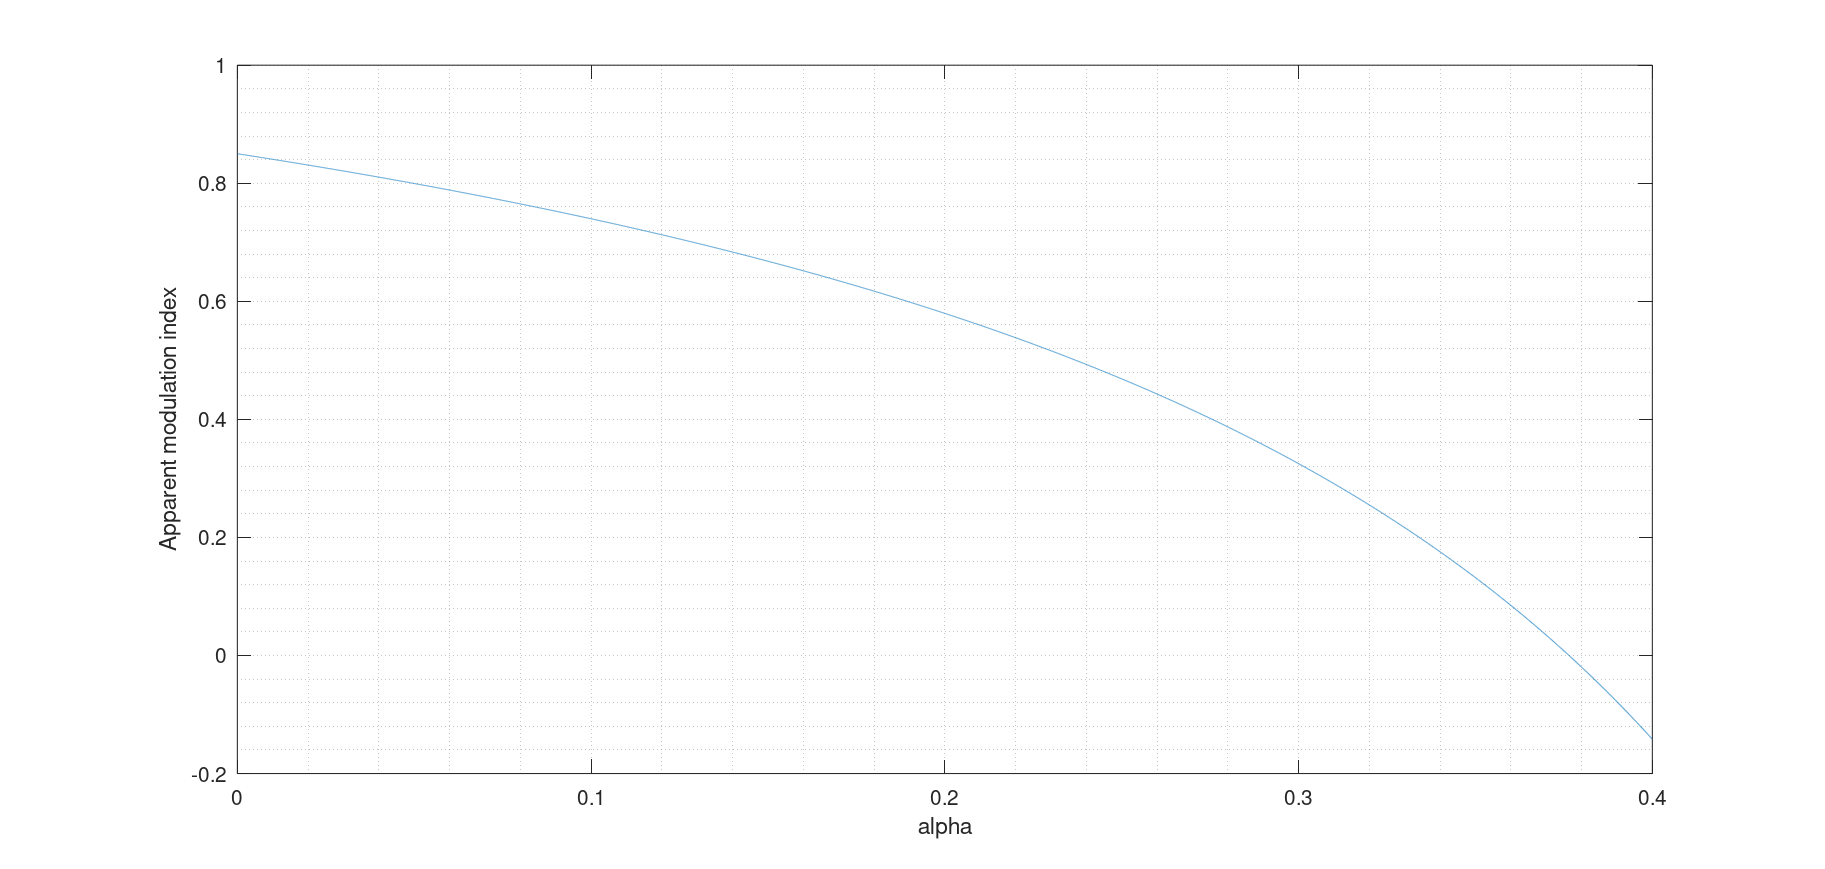
\includegraphics[scale=.25]{app_mod_index_alpha}
\caption{Apparent modulation index vs alpha-parameter. [TODO: Add units]}
\end{figure}

Note how the apparent modulation index is zero at $\alpha = \alpha_0$, as predicted.

Inserting the expression for $\alpha$ in terms of $IIP_3$ into Equation (28) yields
\begin{equation}
\begin{aligned}
m_{eff} &= m \frac{1 - \frac{4}{3 IIP_3^2} \frac{9 m^2 + 36}{16}}{1 - \frac{4}{3 IIP_3^2} \frac{36 m^2 +24}{32}} \\
        &= m \frac{IIP_3^2 - \frac{3}{4} m^2 - 3}{IIP_3^2 - \frac{3}{2} m^2 - 1} \\
\end{aligned}
\end{equation}
There is obviously a singularity at $IIP_3 = \sqrt{\frac{3}{2} m^2 + 1}$ ($\simeq 1.4435$ for $m = 0.85$), and a zero at $IIP_3 = \sqrt{\frac{3}{4} m^2 + 3}$ ($\simeq 1.8820$ for $m = 0.85$).

Furthermore, plotting $m_{eff}$ versus $IIP_3$ yields Figure 2.
\begin{figure}[!h]
\centering
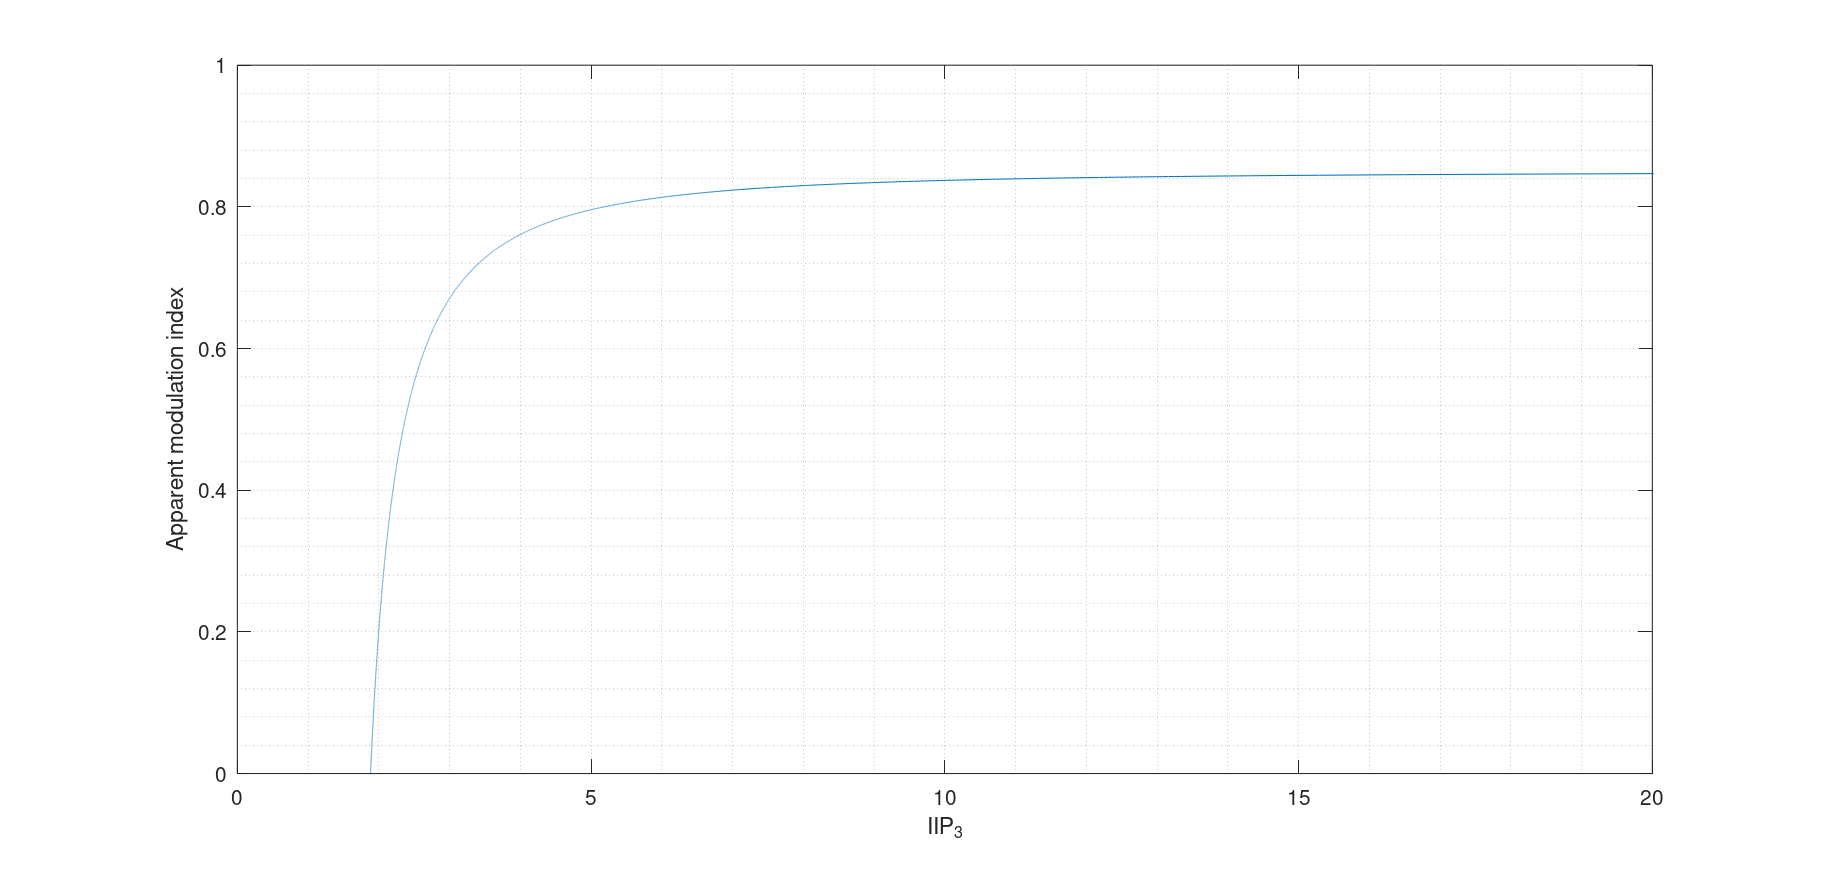
\includegraphics[scale=.25]{app_mod_index_iip3}
\caption{Apparent modulation index vs IIP3. Curve at and below singularity not shown. [TODO: Add units]}
\end{figure}
From the figure, it appears that to avoid noticeable modulation index degradation, ist best to keep $IIP_3 > 10 $V,
corresponding to $(10V)^2 / 1\Omega =$ 100 W in a $1 \Omega$ system, or 2 W in a $50 \Omega$ system.


{\tiny \begin{center} End of document \end{center}}

\end{document}
